% Document packages / layout
\documentclass[12pt]{article}

% --------------------------------------------------------------
% Abhi's Standard math Preamble.
% --------------------------------------------------------------

% Beauty Packages
\usepackage[margin=1in]{geometry} %1 inch margins
\usepackage{color}
\usepackage[final]{microtype}
\emergencystretch=1em

%% Linking Packages
\PassOptionsToPackage{hyphens}{url}
%\usepackage[plainpages=false, colorlinks=true, allcolors=red]{hyperref}
\usepackage[plainpages=false, allcolors=red]{hyperref}

% Math Packages
\usepackage{amsmath,amsthm,amssymb}
\usepackage{commath} %for \norm and \abs
\usepackage{bm}
\usepackage{dsfont}
\usepackage{mathtools}
\usepackage{mathrsfs}
\usepackage{physics}
\usepackage{stmaryrd}
\usepackage{xfrac}
\allowdisplaybreaks

% Quality of Life Packages
\usepackage{enumitem} %styles of enumeration
\usepackage{ulem} %strikethrough
\usepackage{pgffor}
\usepackage{booktabs} %Better quality tables
\usepackage{float} %H option for figures

% Bibliography Packages
\usepackage[backend=biber, style=alphabetic]{biblatex}
\addbibresource{citations.bib}
\usepackage{breakcites}

% Aliases and Package Settings
%% Operator aliases
\newcommand{\mc}[1]{\mathcal{#1}}
\newcommand{\mb}[1]{\mathbb{#1}}
%% Set aliases
\newcommand{\C}{\mathbb{C}}
\newcommand{\N}{\mathbb{N}}
\newcommand{\Z}{\mathbb{Z}}
\newcommand{\Q}{\mathbb{Q}}
\newcommand{\R}{\mathbb{R}}
%% analysis aliases
\newcommand{\e}{\varepsilon}
\DeclarePairedDelimiterX{\inp}[2]{\langle}{\rangle}{#1, #2}
%% Matrix aliases
\newcommand{\T}{\mathrm{T}}
\renewcommand{\vec}[1]{{\mathchoice
                     {\mbox{\boldmath$\displaystyle{#1}$}}
                     {\mbox{\boldmath$\textstyle{#1}$}}
                     {\mbox{\boldmath$\scriptstyle{#1}$}}
                     {\mbox{\boldmath$\scriptscriptstyle{#1}$}}}}
\newcommand{\mat}[1]{\mathbf{{#1}}}
% Chertock aliases
\newcommand*\xbar[1]{%
  \hbox{%
    \vbox{%
      \hrule height 0.5pt % The actual bar
      \kern0.15em%         % Distance between bar and symbol
      \hbox{%
        \kern-0.1em%      % Shortening on the left side
        \ensuremath{#1}%
        \kern-0.0em%      % Shortening on the right side
      }%
    }%
  }%
}


\begin{document}
\title{
  A Well-Balanced Stochastic Galerkin Method for PDEs with Random Forcing
}
\author{%
  Abhijit Chowdhary\footnote{%
    Department of Mathematics, North Carolina State University, Raleigh, NC
    27695, USA (\url{achowdh2@ncsu.edu}, \url{ajshedlo@ncsu.edu})
  }\ \ 
  and Andrew Shedlock\footnotemark[1]
}
\date{Last Edited: \today}
\maketitle

%%%%%%%%%%%%%%%%%%%%%%%%%%%%%%%%%%%%%%%%%%%%%%%%%%%%%%%%%%%%%%%%%%%%%%%%%%%%%%%%
%%% Introduction
%%%%%%%%%%%%%%%%%%%%%%%%%%%%%%%%%%%%%%%%%%%%%%%%%%%%%%%%%%%%%%%%%%%%%%%%%%%%%%%%
\section{Introduction}
In this past couple of decades, the field of Uncertainty Quantification has grown significantly.
Indeed, many of the models we use in the study of numerical methods for them are just that, models derived from some physical process.
Most of the time we use idealized examples which ignore some uncertainty in the given parameters under the assumption that they would negligible, but work in the field has proven that to either be untrue, or for those uncertain parameters themselves to the be the quantities of interest.
Hence, there is a real need for numerical methods correctly propagating uncertainties.

Of particular interest are PDE-based systems with random forcing, for example bottom topographies in systems describing shallow waters. Taking a simplified 1D model of it, we consider systems of the form
\begin{equation}
    \label{eq:Intro-PDE}
    u_t + f(u)_x = -b'(x,z) q(u)
\end{equation}
where $z$ is distributed according to some random variable and is the uncertainty we seek to resolve in the solution.
In \cite{Xiu2002, Xiu2010}, the Stochastic Galerkin method, which is a traditional Galerkin method with orthogonal basis given by a generalized polynomial chaos (gPC) expansion in the random variable space, was constructed and is a viable scheme to solve \eqref{eq:Intro-PDE}.
However, even in the deterministic case, numerical schemes for equations such as \eqref{eq:Intro-PDE} need to be built with care should we want them to resolve the steady state solution; low regularity in the source can destroy the accuracy of traditional solvers.
This is desirable, as much of the study of such equations revolve around understanding small perturbations of the steady state, and whether or not it is stable to such perturbations.
Well-balanced schemes which preserve the steady state have been well studied, and in \cite{Jin2001} they constructed what they called the \textit{interface method} which preserved the steady state of the deterministic version of \eqref{eq:Intro-PDE}.

The goal of this report is to investigate the results of the paper \cite{Jin2015}, which took the traditional gPC stochastic Galerkin method and the well balanced interface method and constructed a well balanced stochastic Galerkin (SGWB) method, which, to our knowledge, was the first such paper to employ such a technique.
As the extension of such ideas are of current research interest, the verification of the reproducability of the results is an important task.
In section 2 we will lay out the theory for the construction of such a SGWB method, and in section 3 we will reconstruct the figures found in the original paper.

%%%%%%%%%%%%%%%%%%%%%%%%%%%%%%%%%%%%%%%%%%%%%%%%%%%%%%%%%%%%%%%%%%%%%%%%%%%%%%%%
%%% Methods
%%%%%%%%%%%%%%%%%%%%%%%%%%%%%%%%%%%%%%%%%%%%%%%%%%%%%%%%%%%%%%%%%%%%%%%%%%%%%%%%
\section{Methods}
As we described in the introduction, the scheme we will satisfy both a well-balanced condition and a stochastic Galerkin projection condition. In the deterministic case We are working a system of the form
\begin{align}
    u_t + f(u)_x &= -b'(x)u \label{PDE}
\end{align}
At the steady state we have that $u_t = 0$, and $(\ref{PDE})$ becomes the steady state condition
\begin{align}
    f(u)_x +b'(x)u &= 0 \label{ss}
\end{align}
We limit our discussion to when $f(u) = \frac{u^2}{2}$ and $f(u) = \frac{u^4}{4}$ to highlight the central idea. For these two choices of $f$, we have that $\frac{f'(\xi)}{\xi}$ is a well-defined number for all $\xi$. We can now define an operator $D:\mathbb{R}\to\mathbb{R}$ by
\begin{align*}
    D(u) &= \int_0^{u}\frac{f'(\xi)}{\xi}d\xi
\end{align*}
Now if $u(x)$ is a strong solution to $(\ref{ss})$ and $u > 0$, then by Liebniz rule
\begin{align*}
    D(u(x))_x + b'(x) &= \frac{f'(u(x))u_x}{u(x)} + b'(x) = \frac{f(u(x))_x}{u(x)} + b'(x) = 0
\end{align*}
This shows that if $u$ is a strong solution to $(\ref{ss})$ and $u > 0$, then $D(u(x)) + q(x)$ is equal to some constant. If we assume that $D(u(x))_x\not=0$, then we can see that
\begin{align}
    u(x) &= \frac{f(u)_x}{D(u(x))_x}\label{u(x)}
\end{align}
Equation $(\ref{u(x)})$ will come into play shortly, but first we must introduce our notation for the discrete system. If we adopt the finite volume framework, then we shall have $N_x$ cells with uniform mesh size of $\Delta x$. For $j = 1, \ldots, N_x$, we let $x_j$ represent the point at the center of the cell and let $x_{j+1/2}$ represent a point at a cell interface. Since we will have a uniform mesh, then $\Delta x = x_{j+1/2}-x_{j-1/2}$. We also have a uniform discretization in time and let $t^n$ represent the discretization at then $n^{th}$ level and $\Delta t =t^{n}-t^{n-1}$. The cell average at $t^n$ over $[x_{j-1/2},x_{j+1/2}]$ is given by
\begin{align*}
    u_j^n &= \frac{1}{\Delta x}\int_{x_{j-1/2}}^{x_{j+1/2}} u(x,t^n)dx
\end{align*}
At the cell interfaces we will have
\begin{align*}
    &D_{j+1/2} = D(u_{j+1/2})
    &&f_{j+1/2}= f(u_{j+1/2})
    &&&b_{j+1/2} = b(x_{j+1/2})
\end{align*}
Now the value $u_{j+1/2}$ can be computed at the cell interface by using either a Godunov scheme or a Roe scheme. Under this finite volume framework, $(\ref{u(x)})$ can be approximated as
\begin{align*}
    u_j^n &\approx \frac{\frac{f_{j+1/2}-f_{j-1/2}}{\Delta x}}{\frac{D_{j+1/2}-D_{j-1/2}}{\Delta x}} = \frac{f_{j+1/2}-f_{j-1/2}}{D_{j+1/2}-D_{j-1/2}}
\end{align*}
This observation leads to the semi-discrete scheme for $(\ref{PDE})$ to be
\begin{align*}
    \partial_tu_j + \frac{f_{j+1/2}- f_{j-1/2}}{\Delta x} &= -\frac{(b_{j+1/2}-b_{j-1/2})}{\Delta x}\Big(\frac{f_{j+1/2}-f_{j-1/2}}{D_{j+1/2}-D_{j-1/2}}\Big)
    \intertext{At the steady state we will get}
    \frac{f_{j+1/2}- f_{j-1/2}}{\Delta x} &= -\frac{(b_{j+1/2}-b_{j-1/2})}{\Delta x}\Big(\frac{f_{j+1/2}-f_{j-1/2}}{D_{j+1/2}-D_{j-1/2}}\Big)\\
    D_{j+1/2}-D_{j-1/2} &= -(b_{j+1/2}-b_{j-1/2})\\
    D_{j+1/2}+b_{j+1/2} &= D_{j-1/2}+b_{j-1/2} = \text{constant}
\end{align*}
In particular for the Burgers' equation we have that $f(u) = \frac{u^2}{2}$, so $D(u) = u$ and so
\begin{align*}
    \frac{f_{j+1/2}-f_{j-1/2}}{D_{j+1/2}-D_{j-1/2}} &= \frac{u_{j+1/2}^2 - u_{j-1/2}^2}{2(u_{j+1/2}-u_{j-1/2})} = \frac{u_{j+1/2}+u_{j-1/2}}{2}
\end{align*}
It follows that the following semi-discrete method for the Burgers' equation is well-balanced. 
\begin{align}
    \partial_t u_j + \Big(\frac{u_{j+1/2}^2-u_{j-1/2}^2}{\Delta x}\Big) &= -\Big(\frac{b_{j+1/2}-b_{j-1/2}}{\Delta x}\Big)\Big(\frac{u_{j+1/2}+u_{j-1/2}}{2}\Big)\label{semidiscrete_burgers}
\end{align}
It is described in \cite{Jin2001} that for a general $f$ that the scheme is well balanced. 
\begin{align}
    \partial_t u_j + \Big(\frac{f_{j+1/2}-f_{j-1/2}}{\Delta x}\Big) &= -\Big(\frac{b_{j+1/2}-b_{j-1/2}}{\Delta x}\Big)\Big(\frac{u_{j+1/2}+u_{j-1/2}}{2}\Big) \label{deterministic_wb}
\end{align}
This gives us the formulation for the deterministic well-balancing. We will incorporate this condition into the general condition for the scheme.\\ \newline
For the stochastic case, we incorporate some uncertainty into our bottom topography via a random variable $z:\Omega\to\mathbb{R}$ with law $P$. For every instance of our random variable $z$, let $u(x,t;z)$ be the function $(x,t)\to u(x,t;z)$ which solves
\begin{align}  \label{Stochastic_PDE}
    u_t(x,t;z) + f(u(x,t;z))_x &= - b(x;z)u(x,t;z)
\end{align}
If we suppose that we have appropriate integrability conditions so that $u(x,t;z),z\in L^2(P)$ holds for all $(x,t)$, then we can use that $u(x,t;z)$ will be $z-$measurable. Consider $$\mathcal{P} = \{\phi(z):\,\phi\,\,\text{is a polynomial of any order}\}$$ 
Then $\mathcal{P}$ is a dense vector subspace in the space of all $z-$measurable functions. Since $\mathcal{P}\subset L^2(P)$ by our integrability assumption on $z$ and that $L^2(P)$ is a Hilbert space, then we can find an orthonormal basis $\{\Phi_m(z)\}_{m\in\mathbb{N}}$ of $\mathcal{P}$. Thus $\{\Phi_m(z)\}_{m\in\mathbb{N}}$ is dense in the space $z-$measurable functions. Then since $u(x,t;z)$ is $z-$measurable, then we can find coefficients $\hat{u}_m(x,t)$ such that $P-$almost everywhere we have that
\begin{align}
    u(x,t;z) &= \sum_{m\in\mathbb{N}}\hat{u}_m(x,t)\Phi_m(z)&&\hat{u}_m(x,t) = \mathbb{E}[u(x,t;z)\Phi_m(z)]\nonumber\\
    b(x;z) &= \sum_{m\in\mathbb{N}}\hat{b}_m(x)\Phi_m(z)&&\hat{b}_m(x) = \mathbb{E}[b(x;z)\Phi_m(z)]\nonumber
\end{align}
We want $(\ref{Stochastic_PDE})$ to hold for almost every instance of our random variable. Since $\{\Phi_m(z)\}_{m\in\mathbb{N}}$ forms an orthonormal basis, this is equivalent to enforcing the condition
\begin{align}
    \mathbb{E}[(\partial_tu(x,t;z) &+ f(u(x,t;z))_x)\Phi_m(z)] = \mathbb{E}[-b'(x,z)u(x,t;z)\Phi_m(z)] \label{stochastic_condition}
\end{align}
for all $m\in\mathbb{N}$. In the discrete setting, we can only take a finite number of basis elements, so let $N$ represent the number of nodes that we are considering. Then the galerkin approximation of $u$ and $b$ in terms of $z$ is given by
\begin{align*}
    u_N(x,t;z) &= \sum_{m=1}^{N+1}\hat{u}_m(x,t)\Phi_m(z)\\
    b_N(x;z) &= \sum_{m=1}^{N+1}\hat{b}(x)\Phi_m(z)
\end{align*}
If we fix $t$, then let $u_{N,j} = u_N(x_j,t;z)$ where the right hand side is the cell average over $[x_{j-1/2},x_{j+1/2}]$. We take $u_{j+1/2}\approx u_j$ and similarly for the other components to get that with $(\ref{deterministic_wb})$ we have that scheme
\begin{align*}
      \partial_t u_{N,j} + \Big(\frac{f(u_{N,j})-f(u_{N,j-1})}{\Delta x}\Big) &= -\Big(\frac{b_{N,j}-b_{N,j-1}}{\Delta x}\Big)\Big(\frac{u_{N,j}+u_{N,j-1}}{2}\Big) %\label{deterministic_wb}
\end{align*}
If we then enforce the condition $(\ref{stochastic_condition})$, we derive the following condition on the scheme we construct
\begin{align}
    \mathbb{E}\Big[\Big(\partial_t u_{N,j} + \Big(\frac{f(u_{N,j})-f(u_{N,j-1})}{\Delta x}\Big)\Big)\Phi_m(z)\Big] &= -\mathbb{E}\Big[\Big(\frac{b_{N,j}-b_{N,j-1}}{\Delta x}\Big)\Big(\frac{u_{N,j}+u_{N,j-1}}{2}\Big)\Phi_m(z)\Big]\label{condition}
    \intertext{We say that any scheme which satisfies $(\ref{condition})$ for all $m\in\mathbb{N}$, over all cells and for all time is a Well-Balanced Stochastic Galerkin method for $(\ref{eq:Intro-PDE})$. If we set $\mathbf{u}_j = (\hat{u}_{1,j},\ldots,\hat{u}_{N+1,j})^T$, define $\mat{E}$ to be the tensor with components $e_{klm} = \mathbb{E}[\Phi_k\Phi_l\Phi_m]$ and $\mat{D}$ to be the tensor with components $d_{klmnp} = \mathbb{E}[\Phi_k\Phi_l\Phi_m\Phi_n\Phi_p]$ and where $1\leq k,l,m,n,p\leq N+1$. We then define matrices $\mathbf{A}_j,\mathbf{S}_j,\mathbf{B}$ to have components}
    \mathbf{A}_{kl,j} &= \sum_{m=1}^{N+1}e_{klm}\hat{u}_{m,j}\nonumber\\
    \mathbf{B}_{kl,j} &= \sum_{m=1}^{N+1}e_{klm}\hat{b}_{m,j}\nonumber\\
    \mathbf{S}_{kl,j} &= \sum_{m,n,p=1}^{N+1}d_{klmnp}\hat{u}_{m,j}\hat{u}_{n,j}\hat{u}_{p,j}\nonumber
\end{align}
If $f(u) = \frac{u^2}{2}$, then a scheme which satisfies $(\ref{condition})$ is
\begin{align}
    \label{eq:u2-WBSG}
    \partial_t\mathbf{u}_j + \frac{\mathbf{A}_j \mathbf{u}_j - \mathbf{A}_{j-1}\mathbf{u}_{j-1}}{2\Delta x} &=- \frac{(\mathbf{B}_j-\mathbf{B}_{j-1})(\mathbf{u}_j + \mathbf{u}_{j-1})}{2\Delta x}
    \intertext{If $f(u) = \frac{u^4}{4}$, then a scheme which satisfies $(\ref{condition})$ is}
    \label{eq:u4-WBSG}
    \partial_t\mathbf{u}_j + \frac{\mathbf{S}_j \mathbf{u}_j - \mathbf{S}_{j-1}\mathbf{u}_{j-1}}{4\Delta x} &=- \frac{(\mathbf{B}_j-\mathbf{B}_{j-1})(\mathbf{u}_j + \mathbf{u}_{j-1})}{2\Delta x}
\end{align}
%%%%%%%%%%%%%%%%%%%%%%%%%%%%%%%%%%%%%%%%%%%%%%%%%%%%%%%%%%%%%%%%%%%%%%%%%%%%%%%%
%%% Results
%%%%%%%%%%%%%%%%%%%%%%%%%%%%%%%%%%%%%%%%%%%%%%%%%%%%%%%%%%%%%%%%%%%%%%%%%%%%%%%%
\section{Results}
In order to verify that the proposed methods satisfy the well-balanced claim, in this section we provide several numerical examples of it doing so.
Consider the stochastic PDE \eqref{Stochastic_PDE} that we constructed methods for last section; imposing the boundary conditions:
\[
\begin{cases}
    u(x,0) = 0, &\text{for } x > 0 \\
    u(0,t) = 2, &\text{for } t > 0
\end{cases}
\]
we solve the PDE under both Burger's flux $f(u) = u^2 /2$ and the alternate flux given by $f(u) = u^4 / 4$ over the following choices of bottom topography:
\begin{align}
    \label{b1}
    b_1(x,z)
    &=
    \begin{cases}
        (2+z) \cos(\pi x), & 4.5 \leq x \leq 5.5 \\
        0, & \text{otherwise}
    \end{cases} \\
    \label{b2}
    b_2(x,z)
    &=
    \begin{cases}
        0.1(2+z) \cos(\pi x), & 5 \leq x \leq 6 \\
        0, & \text{otherwise}
    \end{cases}
\end{align}
Bottom topography \eqref{b1} is continuous whereas \eqref{b2} is discontinuous, resulting in continuous and discontinuous resulting solutions.
In all examples $z \sim {\rm Uniform}[-1,1]$.

For a point of comparison, we compare our method to the so called \textit{cell-average} method:
\begin{align}
    \label{eq:cell-average-u2}
    \partial_t\vb{u}_j + \frac{\mat{A}_j \vb{u}_j - \mat{A}_{j-1}\vb{u}_{j-1}}{2\Delta x} &=- \frac{(\mat{B}_j-\mat{B}_{j-1})}{\Delta x}\vb{u}_j \\
    \label{eq:cell-average-u4}
    \partial_t\vb{u}_j + \frac{\mat{S}_j \vb{u}_j - \mat{S}_{j-1}\vb{u}_{j-1}}{2\Delta x} &=- \frac{(\mat{B}_j-\mat{B}_{j-1})}{\Delta x}\vb{u}_j
\end{align}
where \eqref{eq:cell-average-u2} corresponds to the flux $f(u) = u^2 / 2$ and $\eqref{eq:cell-average-u4}$ corresponds to $f(u) = u^4 / 4$, and matrices $\mat{A}, \mat{B}, \mat{S}$ are as described above.


For all simulations, we choose number of cells $N_c = 100$, time step fixed to $\Delta t = 3200^{-1}$, and we integrate to final time $T = 10$. 
In the steady state, assuming $u > 0$, \eqref{Stochastic_PDE} reduces down to $u'(x) = -b'(x,z)$, hence we find the steady state solution $u(x) = 2 - b(x,z)$, from which we can derive the steady state mean and standard deviation $\mathbb{E}[u] = 2 - 2b(x,0)$ and $\mathbb{V}[u] = \frac{1}{\sqrt{3}} |b(x,0)|$, which is what we compare the numerically computed solution to in Figure \ref{fig:b1} and similar in Figure \ref{fig:b2}.
However, when a true mean and variance aren't available for comparison, for example with flux $f(u) = u^4 / 4$, one is numerically integrated for instead.

The results of these tests, found in Figures \ref{fig:b1}, \ref{fig:b2} and \ref{fig:u4}, ultimately verify the fact that our scheme is Well-Balanced and offers a significant accuracy improvement naive cell-average scheme. 
Furthermore, a convergence study was done varying in both gPC-order and number of cells, where we verified that the method was indeed first-order convergent in space, see Figure \ref{fig:convergence}. 
It also verified the expected conclusion that the errors in the random space saturate extremely quickly, as in both $b_1$ and $b_2$ are of order $\mc{O}(z)$.

Finally, one can view table \ref{tab:cpu-time} for a time estimates for running the given method, varying in both $N_c$ and gPC-order. 
Indeed, getting these times down to their current level was not a trivial computational task, initial versions of the code would take around 120 seconds with $N_c = 100$ and $4$ gPC coefficients.
Algorithmic improvements primarily through exploiting symmetry in $\mat{A}$ and $\mat{S}$ reduced the wall time down to around 50 seconds, but an eventual rewrite from MATLAB into Julia and exploiting its capabilities in avoiding unnecessary allocations and pre-compilation as opposed to a JIT system resulted in the final time of around 4 seconds, with around 4 additional seconds for compilation.

\begin{table}[!htb]
\centering
\begin{tabular}{@{}l|lll@{}}
\toprule
CPU Time & 100  & 200  & 400   \\ \midrule
1        & 2.83 & 3.62 & \ 7.28  \\
2        & 2.84 & 5.69 & 11.22 \\
3        & 3.14 & 6.07 & 12.22 \\
4        & 3.81 & 7.64 & 15.37 \\ \bottomrule
\end{tabular}
\caption{The estimated CPU time (seconds) for the Well-Balanced Stochastic Galerkin method for bottom topography $b_1$ and flux $f(u) = u^2/2$ with cell count $N_c \in \{100, 200, 400\}$ and number of gPC coefficients $M \in \{1,2,3,4\}$.}
\label{tab:cpu-time}
\end{table}

\begin{figure}[!htb]
    \centering
    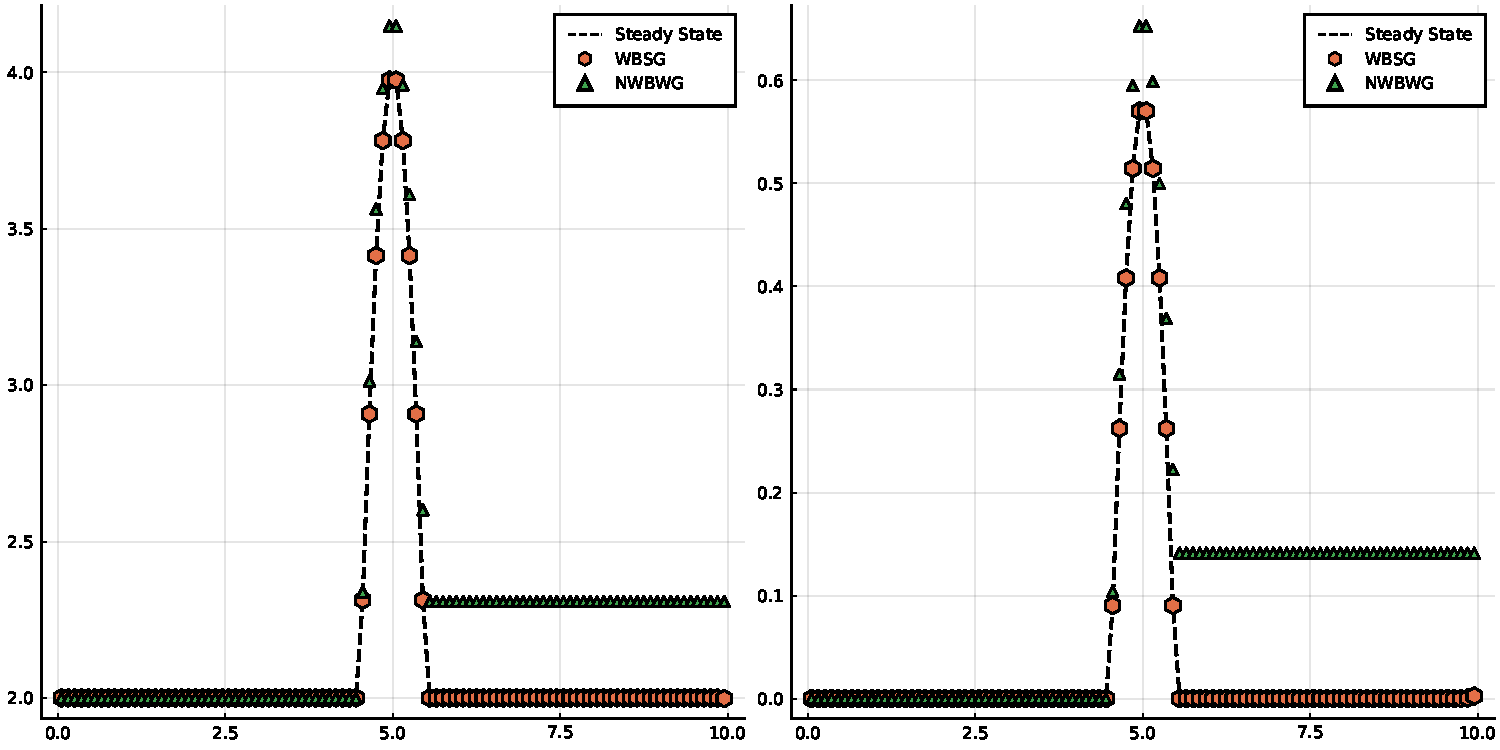
\includegraphics[width=0.95\textwidth]{Figures/b1}
    \caption{The results of the constructed WBSG (circles) \eqref{eq:u2-WBSG} versus the non-WBSG method (triangles) \eqref{eq:cell-average-u2} with forcing $b_1$. We use $N_c = 100$ cells and limit ourselves to a 4th order gPC expansion. On the left is a graph of the computed mean and on the right is the computed standard deviation. Indeed, we find that the new method resolves the steady state correctly.}
    \label{fig:b1}
\end{figure}
\begin{figure}[!htb]
    \centering
    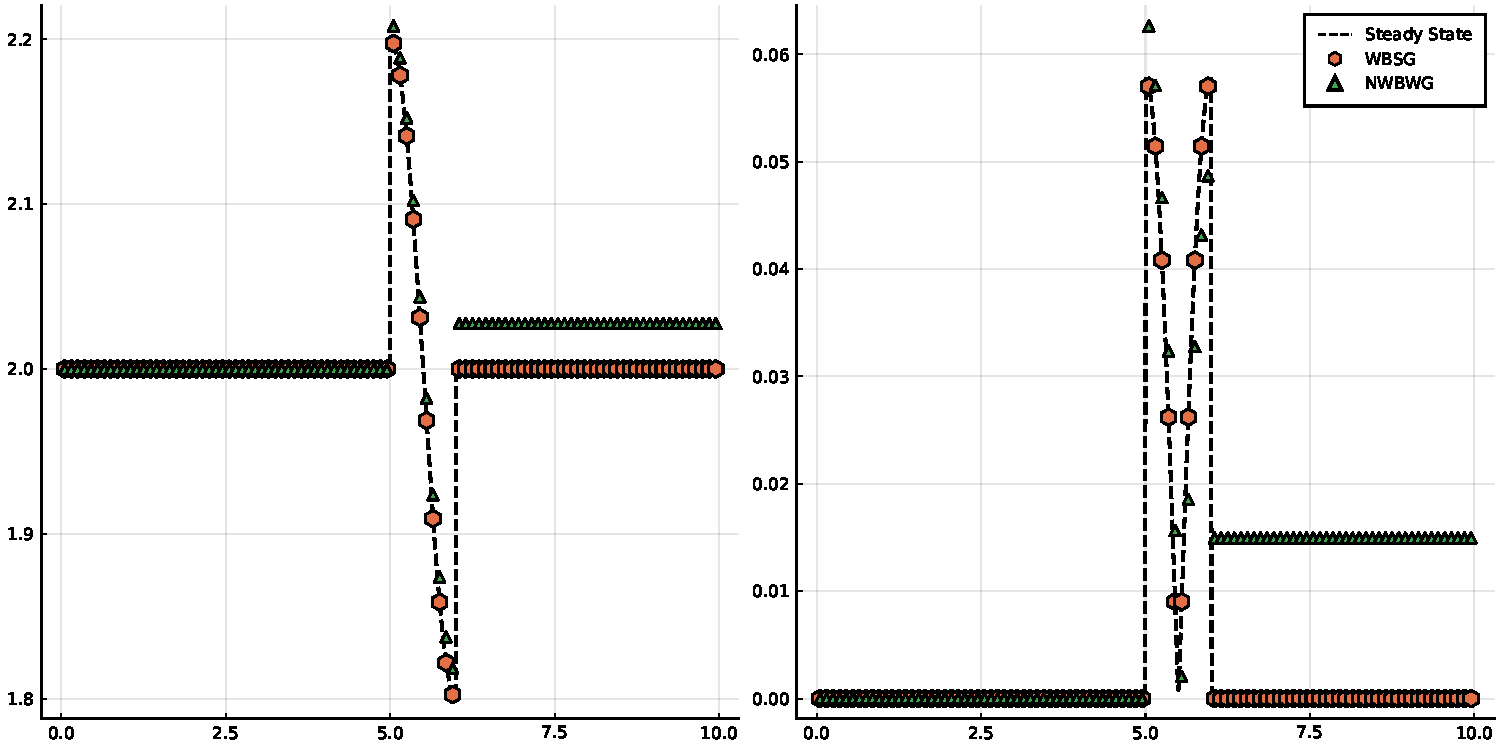
\includegraphics[width=0.95\textwidth]{Figures/b2}
    \caption{The results of the constructed WBSG (circles) \eqref{eq:u2-WBSG} versus the non-WBSG method (triangles) \eqref{eq:cell-average-u2} with forcing $b_2$. We use $N_c = 100$ finite volume cells and limit ourselves to a 4th order gPC expansion. On the left is a graph of the computed mean and on the right is the computed standard deviation. Indeed, we find that the new method resolves the steady state correctly even in the discontinuous case.}
    \label{fig:b2}
\end{figure}
\begin{figure}[!htb]
    \centering
    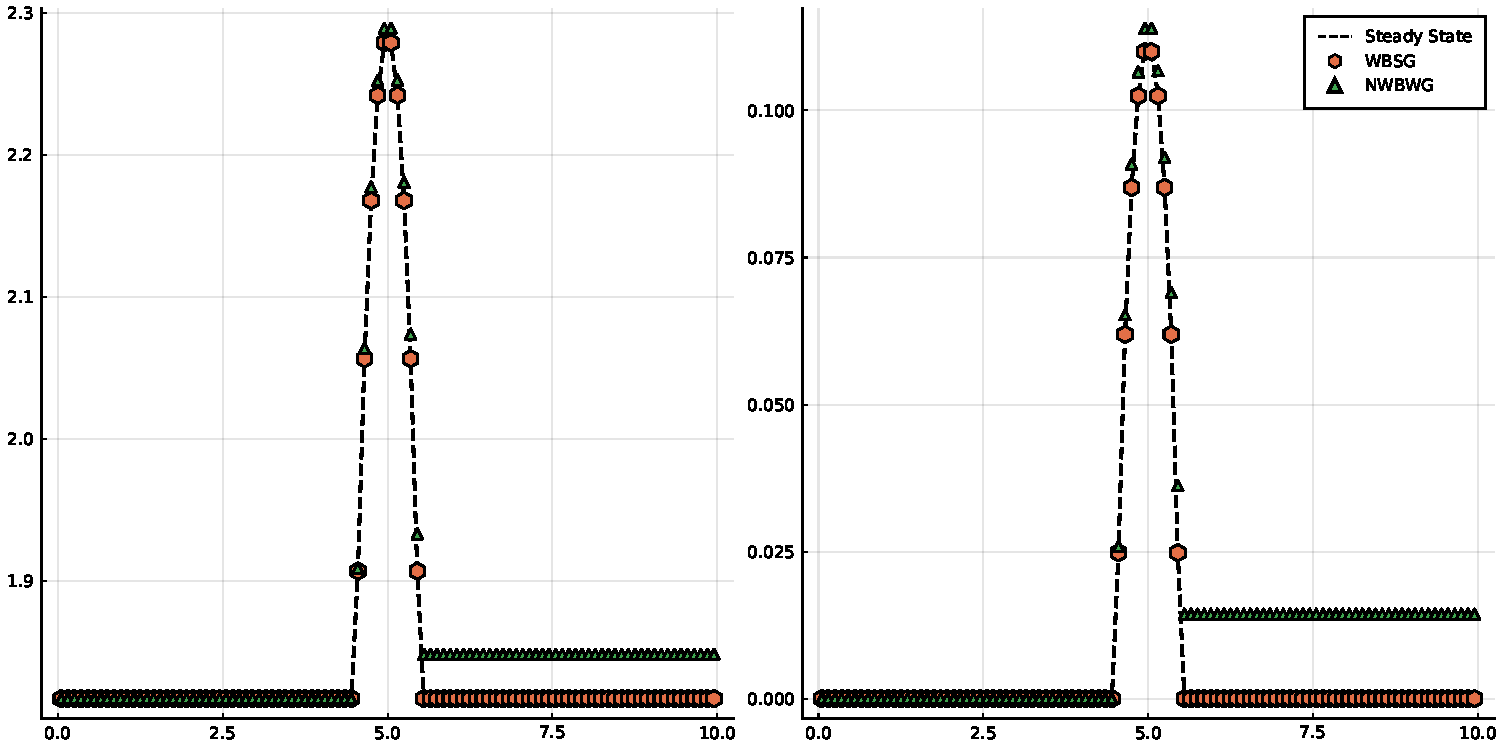
\includegraphics[width=0.95\textwidth]{Figures/u4}
    \caption{The results of the constructed WBSG (circles) \eqref{eq:u4-WBSG} versus the non-WBSG method (triangles) \eqref{eq:cell-average-u4} with forcing $b_1$. We use $N_c = 100$ finite volume cells and limit ourselves to a 4th order gPC expansion. On the left is a graph of the computed mean and on the right is the computed standard deviation. Indeed, we find that the new method resolves the steady state correctly even for alternative fluxes.}
    \label{fig:u4}
\end{figure}
\begin{figure}[!htb]
    \centering
    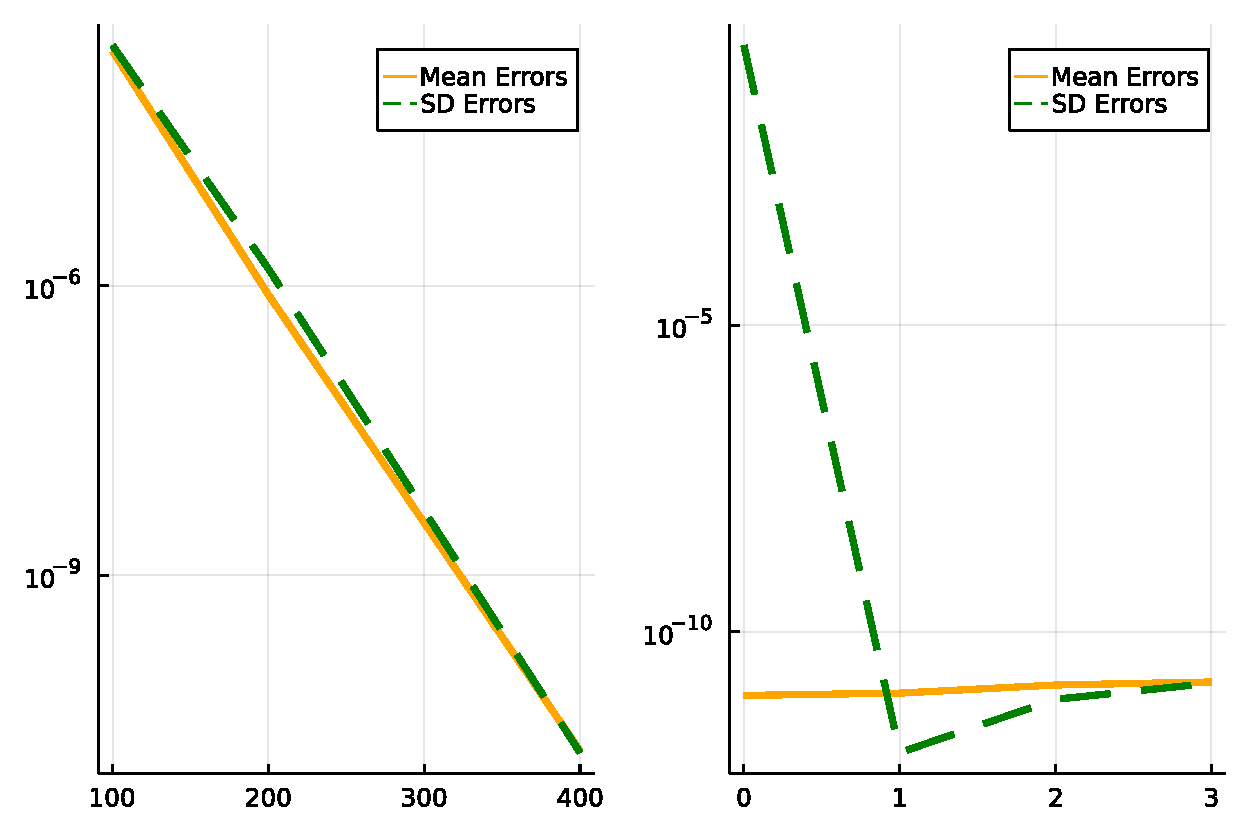
\includegraphics[width=0.95\textwidth]{Figures/convergence}
    \caption{This figure denotes the convergence results for \eqref{eq:u2-WBSG} with forcing $b_1$. The figure on the left denotes convergence in space with a 4th order gPC expansion, and the figure on the right denotes convergence in the order of the gPC expansion holding the spatial discretization at $N_c = 800$. Indeed we verify that our method is spatially of first order, and that it took only 2 gPC coefficient to resolve the uncertainties.}
    \label{fig:convergence}
\end{figure}

%%%%%%%%%%%%%%%%%%%%%%%%%%%%%%%%%%%%%%%%%%%%%%%%%%%%%%%%%%%%%%%%%%%%%%%%%%%%%%%%
%%% Conclusion
%%%%%%%%%%%%%%%%%%%%%%%%%%%%%%%%%%%%%%%%%%%%%%%%%%%%%%%%%%%%%%%%%%%%%%%%%%%%%%%%
\section{Conclusion}
In conclusion, we've verified the results presented in \cite{Jin2015}, i.e. we've taken the well-balanced scheme constructed in \cite{Jin2001} and and extended it to a stochastic setting with the gPC stochastic Galerkin method. 
This is a proof of concept for taking previously constructed deterministic well-balanced schemes and forming Galerkin via gPC methods from them which are well balanced in a stochastic sense, and in theory this should work in general.
This is useful as, in comparison to stochastic collocation methods which can preserve the well-balanced property and the collocation nodes, but struggle to preserve it between them in the interpolation step, these intrusive methods preserve steady state in a weak sense over the whole spatial domain.
As an example, 2 years after this paper was published, \cite{Wu2017} produced an extension of this idea for quasilinear PDEs whose gPC-system may not be hyperbolic.

However, the difficulties of this method ought to be noted.
Outside of the difficulty casting flux's not of the form $f^p(u) = u^p / p$ into this method, it is clear through the construction of $\mat{S}$ in the case of $f(u) = u^4 / 4$ that this method suffers from the curse of dimensionality in gPC-order.
At each time iteration, one must iterate the gPC-coefficients of $\vb{u}$ at each spatial point, resulting in an $N_c \times M$ system to integrated.
This is reasonable for problems with 1 spatial dimension, or with random effects that require few gPC-order to resolve, but as your problem increases in spatial dimension or has increasingly nonlinear random effects the size of coefficients being integrating may grow to be too large.
This is ignoring multi-dimensional random variables, who would case the size of the space $\mathcal{P}_z$ to suffer combinatorial explosion.
This is, of course, intractable, and methods to resolve these dimensionality troubles remain a further area of research.

%%%%%%%%%%%%%%%%%%%%%%%%%%%%%%%%%%%%%%%%%%%%%%%%%%%%%%%%%%%%%%%%%%%%%%%%%%%%%%%%
%%% References
%%%%%%%%%%%%%%%%%%%%%%%%%%%%%%%%%%%%%%%%%%%%%%%%%%%%%%%%%%%%%%%%%%%%%%%%%%%%%%%%
\printbibliography
\end{document}